\documentclass{tufte-handout}
\usepackage{graphicx}
\graphicspath{ {./images/} }

\title{Linear Models of Classification}
\author{Andres Ponce}
\begin{document}
\maketitle
\begin{abstract}
	The goal with \textbf{classification} is "to take 
	an input vector $x$ and to assign it to one of $K$
	discrete classes.
\end{abstract}

If we want to classify a certain input vector, we would have 
to map it to a certain region of a plane, defined by certain 
boundaries.\footnote{Is this similar to \textbf{linear programming},
where we had to optimize a linear combination of the parameters?}

If there are $D$ varaiables we are trying to optimize, then our 
answer will exist in a $D$ dimensional space. 
\subsection{Discriminants}
\textbf{Linear} discriminants can be of the form\footnote{Here, 
$w$ is the parameters, and $w_{0}$ is the bias.}
\[ y(x) = w^{T}x + w_{0}\]
We also ahve a \textbf{decision boundary}, where we know which of the
$K$ categories our input belongs to given our discriminant function,
and a certain cutoff value $C_{x}$.

We can also use a Bayesian approach to determine classification, if we 
calculate $p(C_{k}|x)$\footnote{The probability that given input $x$, 
it belongs in class $k$.}
\begin{marginfigure}
	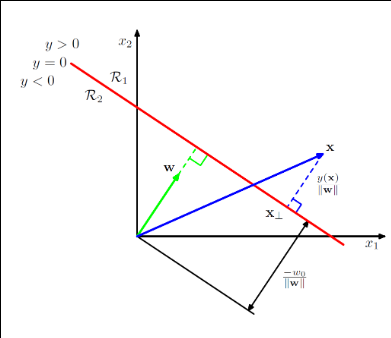
\includegraphics[width=\linewidth]{dec_boundary}
	\caption{The dotted green and blue lines are the 
		distance between the arbitrary point and the 
		decision boundary.}
\end{marginfigure}

How do we extend a linear discriminant to other classes? We can have
\textbf{One-vs-the-rest} or \textbf{one-vs-one} qualifiers.
\subsection{One-vs-the-rest}
	With this type of classifier functions, we try to distinguish those
	inputs on a binary case by case basis. That is, we try to one at a time
	build a classifier that knows points in $C_{i}$ from those points in other
	classes. However, when two points  "not in their repsective classes" fall
	in the same area, this area would be defined differently by the areas we're 
	actually testing.
	\begin{marginfigure}
		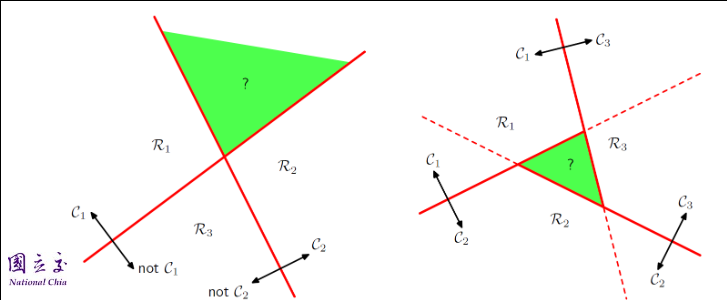
\includegraphics[width=\linewidth]{ambiguous}
		\caption{When a point is not in a certain region, it can 
			be ambiguous where it falls, if the same point can be thought
			of differently by each region.}
	\end{marginfigure}
\subsection{K-class discriminant}
	If we use $K$ linear functions of the form 
	\[ y_{k}(x) = w^{T}_{k}(x) + w_{k0}\]
	Then point x goes in class $k$ iff $y_{k}(x) > y_{j}(x) \forall j\neq k$ 
	\footnote{essentially we describe every region by its own equation, and assign
		the points to the one that fits the best.}
\subsection{Least Squares for classification}
	Similar to the original least squares definition, we want to minimize the difference
	between the data points and the final values. 

	The actual formula for the least squares classification is
	\[ y(x) = \widetilde{W}^{T}\tilde{x}\]

	However, the least squares solution usually does not have the best performance, and is 
	sensitive to \textbf{outliers}.
	\begin{marginfigure}
			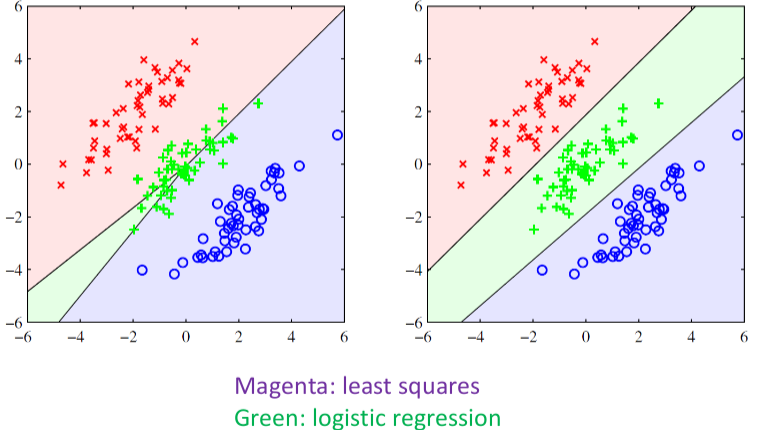
\includegraphics[width=\linewidth]{ls_not_good}
			\caption{Logistic regression can sometimes have better performance than
				ordinary least squares.}
	\end{marginfigure}
\subsection{Fisher's Linear Discriminant:2 classes}
	\textbf{Fisher's Linear Discriminant} can help with dimensionality reduction at the moment
	of solving a K-dimensionality problem. With these kinds of problems, we want to find a lienar
	combinations of elements that maximizes the distance between data points not in the same class.

	That is, we want to reduce the number of dimensions from $D$ down to 1; then we want to select 
	a threshold $t$, which serves to mark where one point would be classified as $C_{1}$ or $C_{2}$.
	After we have clearly separated the different classes in a reduced space, we would like to maximize
	the distance between the points of all classes, so as to minimize the variance between points of the 
	same class and thus maximize the distance between points of different classes.

	The \textbf{mean vectors} between two classes is 
	\[ m_{1} = \frac{1}{N_{1}} \sum_{n\in C_{1}}^{}x_{n}\]
	and likewise for $m_{2}$. Then, we want a function that maximizes the distance between the two
	functions. We would like  
	\[ m_{2} - m_{1} = w^{t}(m_{2} - m_{1})\]
	to be maximized.We also want to minimize the variance within a single class.

	So, if we are trying to determine the variance between the $k$ classes, then we need a way to 
	determine the variance between each of the $k$ classes. Thus, we would calculate something like
	\[s_{k}^{2} = \sum_{n\in C_{k}}^{}(y_{n} - m_{1})\]
	and then repeat this procedure to find out the variance between all the classes.
	\footnote{Remember the \textbf{variance} represents the amount the value differs from the mean. We
	want to minimize the variance between our estimates and the elements of class $k$, but we want to  
	maximize the distance between the means of the two classes when we project onto a single dimension.
	This is the entire feeling behind Fisher's Linear Discriminant.}

	So, there are a coupple ways to carry out classification:
	\begin{itemize}
			\item{Determine a threshold}:We can find a point $x$ such that if $y(x)\geq -y_{0}$,
					$C_{1}$, else $C_{2}$.
			\item{use the nearest-neighbor rule}:When we project a training sample onto a 
					one-dimensional space, we can sample some of the training data a certain 
					distance away, and classifying the point based on the number of training 
					points belonging to a certain class.
	\end{itemize}
	\begin{marginfigure}
			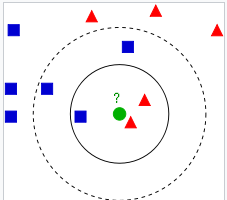
\includegraphics[width=\linewidth]{nearest_neighbors}
			\caption{If we take the sample space to be the solid colored line, we say the green
				sample point is a red triangle, since the closest points are mostly red triangles(2-1).
				Using the dahsed circle, we would classify it as a blue square for the same reason.}
	\end{marginfigure}
\subsection{Perceptron Algorithm}
	The \textbf{perceptron algorithm} works by having a linear combination of the terms 
	$y(x) = f(w^{T}\phi(x))$. We also want $f$ to have a value either $1$ or $-1$. Another
	parameter $t$ can either be set to -1 or 1, and during the training phase we usually set it
	to 1 for $C_{1}$ and -1 for $C_{2}$
	
	The goal of the perceptron then becomes to make $w^{T}\phi(x_{n})t_{n} > 0$, since this means
	that the point $x_{n}$ was correctly classified. In classification problems, we only have a binary
	choice: whether the point was classified into the correct class. Therefore, the error function to 
	judge our model should be a function of all the points that were actually \textit{misclassified}.
	One such function might be
	\[ E_{p}(w) = -\sum_{n\in M}^{}w^{T}\phi_{n}t_{n}\]
	where M is the set of points that were misclassified.
	Then, the weight vector is updated depending on whether we correctly classified the data or not.
	Add $\phi_{n}$ to $w$ if $x_{n}$ belongs to $C_{1}$ and was misclassified, and subtract $\phi_{n}$
	from $w$ if $x_{n}$ belongs to $C_{2}$ and was misclassified.
\subsection{Generative Models}
	In these types of mdoels, we try and figure out $p(C_{k}|x)$ by calculating $p(x|C_{k})$ and $p(C_{k})$
	and solving for Bayes' Theorem.\footnote{The main idea of the gernative model remains to find the 
	\textit{joint probability} both the target variable and our input variable, i.e. $p(t,x)$}

	However, this was only the case for 2 classes; we can try to generalize to more classes. The basic
	formula still very much resembles Bayes' Theorem.\footnote{basically the probability that the input
	vector belongs to class $C_{k}$ over the probability that it belongs to any of the other classes.}
	\[ p(C_{k}|x) = \frac{p(x|C_{k})p(C_{k})}{\sum_{j}^{}p(x|C_{j})p(C_{j})}\]

	With this type of model, we also have to set several parameters, $\pi, \mu_{k}$. \footnote{We can
	use the maximum likelihood to identify the parameters, if we recall by maximizing the log of the 
	likelihood function.}
\subsection{Different models}
	So far, we have two different models for estimating the parameters.
	\begin{itemize}
		\item \textbf{Probabilistic Generative Model}: As we just saw, with this model we try and
				estimate the posterior probability by computing the class priors and trying to 
				solve Bayes' Theorem.
		\item \textbf{Probabilistic Discriminative Models}: Here we also try and solve for the 
				posterior probability of an input belonging to a certain class, but we 
				generalize the linear model (like with Fisher's and Perceptron) to solve for the 
				required parameters directly. There are a couple advantages to using this type
				of model, for example there are less parameters and usually has better performance.
	\end{itemize}
\newthought{After this, the slides mostly just discussed how to find the parameters used in these
and related equations.}
\end{document}
